 \documentclass[a4paper,11pt]{article}
\usepackage[french]{babel}
\usepackage[utf8x]{inputenc}
\usepackage[T1]{fontenc}
\usepackage{caption}
\usepackage{amsmath}
\usepackage{listings}
\usepackage{graphicx}


\usepackage[a4paper,left=2.5cm,right=2.5cm,top=2.5cm,bottom=2.5cm]{geometry}
\usepackage{siunitx}

\title{Assignment1 : Solving problems with uninformed search}

\newenvironment{vcenterpage}
{\newpage\vspace*{\fill}}
{\vspace*{\fill}\par\pagebreak} 

\renewcommand {\arraystretch }{1.5}


\begin{document}
\begin{titlepage}
    \begin{vcenterpage}
\newcommand{\HRule}{\rule{\linewidth}{0.5mm}} 

\center 

\textsc{\LARGE Artificial Intelligence}\\[1.5cm] 
\textsc{\Large \textsc{LINGI2261}}\\[0.5cm] 

\HRule \\[0.8cm]
{ \huge \bfseries Assignment2: Solving Problems with Informed Search}\\[0.4cm] 
\HRule \\[1.5cm]

\begin{minipage}{0.4\textwidth}
\begin{flushleft} \large
\emph{Auteur:}\\
Laurent \textsc{Desausoi}\\
\end{flushleft}
\end{minipage}
~
\begin{minipage}{0.4\textwidth}
\begin{flushright} \large
\emph{Noma:} \\
\textsc{5409-1500}
\end{flushright}
\end{minipage}\\[4cm]

{\large \today}\\[3cm] 

\end{vcenterpage}
\end{titlepage}


\section{Search Algorithms and their relations}
	\subsection{Question 1}
		\par The heuristic I choosed to solve this problem will be later explained in the section 1.4. As for now, I will explain why it is consistent and admissible.
		\par The heuristic is admissible because to compute our heuristic we only use the Manhattan distance and as it never overestimates the distance, the heuristic will never overestimate and is thus admissible. The same conclusion can be easily drawn for the consistent property.
	\subsection{Question 2}
		\begin{figure}[h!]
			\centering
			
\includegraphics[scale=1]{uniform_search}
			\caption{Uninformed search execution}
		\end{figure}
	\subsection{Question 3}
		\begin{figure}[h!]
			\centering
			
\includegraphics[scale=1.35]{astar_search}
			\caption{AStar search execution}
		\end{figure}
	
\section{Pacmen problem}
	\subsection{Question 1}
		\begin{itemize}
			\item States: A state is the configuration of the game at a current time. It consists not only of the positions of the different player but also the internal variable used to compute the heuristic, successor, etc.
			\item Initial state: The initial state is simply the state of the game at the beginning of the game.
			\item Action model: It is simply a model used to represent an action done by a player on the game.
			\item Goal test: The goal test is simply the test that is done at each iteration to check if the game is finished.
			\item Path cost function: The path cost function is the function used to compute the cost to move from one state to an another.
		\end{itemize}
	\subsection{Question 2}
		\par As each pacmen can move at maximum in 4 directions at each iteration, if we have k pacmen, we therefore have a maximum branching factor of $4^k$.
	\subsection{Question 3}
		\par An admissible heuristic would be to compute the sum of the minimum distance between a pacmen and the foods. To compute this value, we first need to look for the closest food from the pacmen and compute the Manhattan distance. We then place the pacmen at the position of the food and repeat the process. We then sum each distances computed and the result gives us the heuristic. The complexity of this heuristic is $\frac{n(n+1)}{2}$, where n is the number of food.
		\par We can affirm that this heuristic is admissible because the Manhattan distance can never be greater than the real distance needed, and we only use the Manhattan distance to compute the heuristic.
	\subsection{Question 4}
		\par For k pacmens, we basically use the same algorithm. The only thing that is different is that the Manhattan distance that we compute is the smallest distance between one of the pacmens and one food. We then move that pacmen to the chosen food and repeat the process as described in Question 3. Its complexity is simply $k\frac{n(n+1)}{2}$.
	\subsection{Question 6}
		\begin{figure}[h!]
			\centering
    		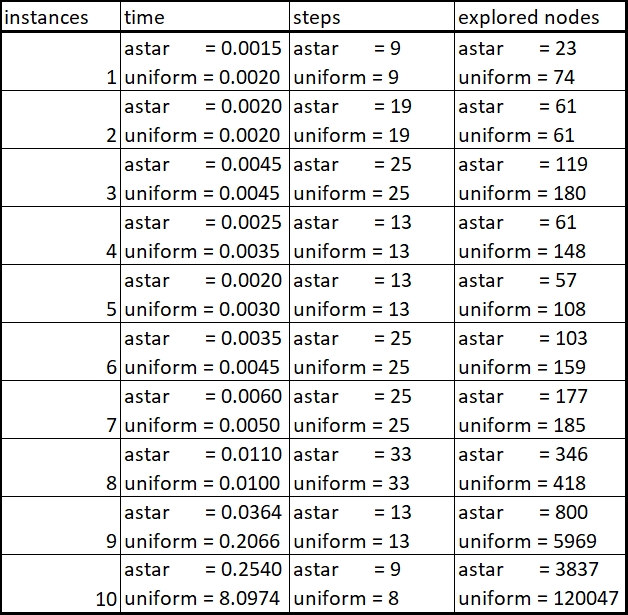
\includegraphics[width=\linewidth]{experiments}
    		\caption{Algorithms experimentations}
		\end{figure}
		\par As we can observe from the experiments, the numbers of nodes explored by the \textit{astar graph} is always less or equals than with the uninformed search. We can also observe that the computation time is not always related to the number of nodes explored. Indeed, we observe that even if the explored nodes of the \textit{uninformed search} is greater than with the \textit{astar search}, it can compute the result faster due to its constant complexity for the heuristic (as it returns always 1).

\end{document}